\begin{minipage}{0.66\linewidth}
    La figure ci-dessous est la reproduction du mouvement du centre d'un mobile
    autoporteur attaché en $O$ fixe sur une table horizontale. L'intervalle de
    temps séparant deux marques consécutives vaut $\tau=\qty{40}{\ms}$.
    
    \begin{enumerate}
        \item Que peut-on dire du mouvement considéré~? Pourquoi~?
              \textbf{(1pt)}
        \item Calculer la vitesse angulaire $\omega_{3}$ du mobile à l'instant
              $t_{3}$ au point $M_{3}$. Préciser l'unité.
              \textbf{(1pt)}
        \item En déduire la vitesse linéaire $v_{3}$ à l'instant $t_{3}$ au point
              $M_{3}$.
              \textbf{(1pt)}
        \item Représenter le vecteur vitesse du mobile aux instants $t_{3}$ et
              $t_{6}$ en utilisant l'échelle~:
              $\qty{1}{\cm} \to \qty{0.1}{\v}$.
              \textbf{(0,5pt)}
    \end{enumerate}
\end{minipage}
\hfill
\begin{minipage}{0.33\linewidth}
    \flushright
        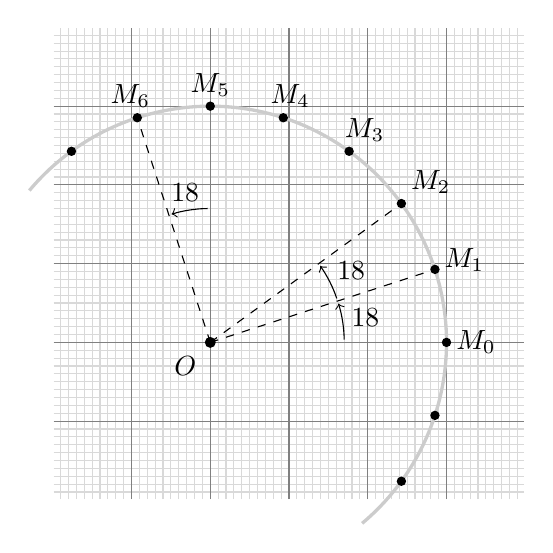
\begin{tikzpicture}
            \def\th{18}
            \newdimen\r \r=3cm
            \draw[step=1mm,black!15] (-1.99,-1.99) grid (3.99,3.99);
            \draw[step=1cm,black!50] (-1.99,-1.99) grid (3.99,3.99);
            \node[inner sep=1.4pt,circle,fill,label=below left:$O$] {};
            \draw[black!20,very thick] (140:\r) arc (140:-50:\r);
            \foreach \a [count=\i from 0] in {0,18,...,140,-36,-18,...,-1}
                \node[circle,inner sep=1.2pt,fill] (M\i) at (\a:\r) {};
            \foreach \i in {0,...,6}
                \node[anchor=180+\i*\th] at (M\i) {$M_{\i}$};
            \draw[dashed] (0,0) -- (M1) (0,0) -- (M2) (0,0) -- (M6);
            \foreach \a in {0, \th, 90}
                \draw[->,shorten <=1pt,shorten >=1pt] (\a:1.7) arc (\a:\a+\th:1.7)
                    node[anchor=180+\a,pos=0.6] {$\qty{18}{\degree}$};
        \end{tikzpicture}
\end{minipage}
